\documentclass[a4paper,12pt]{article}
\usepackage[margin=0.7in]{geometry}
\usepackage[latin1]{inputenc}
\usepackage[english]{babel}
\usepackage{amsmath}
\usepackage{cases}
\usepackage[makeroom]{cancel}
\usepackage{amsmath,tabu}
\usepackage{amsmath}
\usepackage{cases}
\usepackage[makeroom]{cancel}
\usepackage{amsmath,tabu}
\usepackage[fleqn]{mathtools}
\usepackage[fleqn]{amsmath}
\usepackage{bm}
\usepackage{tikz}
\usepackage{enumitem}
\usepackage{wrapfig}
\usepackage{graphicx}
\usepackage{siunitx}
\usepackage{microtype}
\usepackage{array,tabularx}
\usepackage{float}
\usepackage{booktabs}

\title{\textbf{PRECEPT 2}: Heat and mass balances of a steam cycle }
\author{Rossi Andrea 875272}
\date{}

\ExplSyntaxOn
  \cs_new_eq:NN \calc \fp_eval:n
\ExplSyntaxOff
\newcommand*{\formatNumber}[2][]{\num[%
  round-mode=places,% Round output to specified number of places
  round-precision=2,% Round-precision is 3
  output-decimal-marker={.},% Use , as decimal marker
  #1% Other options
  ]{\calc{#2}}}

\newcommand{\celsius}[0]{\,^{\circ}C}
%\newcommand{\bar}[0]{\,bar}
\newcommand{\kjkg}[0]{\,\frac{kJ}{kg}}
\newcommand{\kjkgk}[0]{\,\frac{kJ}{kg \cdot K}}
\newcommand{\kgmcube}[0]{\,\frac{kg}{m^3}}
\newcommand{\kgs}[0]{\,\frac{kg}{s}}
\newcommand{\kw}[0]{\,kW}
\newcommand{\mw}[0]{\,MW}
\newcommand{\md}[0]{Mollier diagram }

\newcommand{\pointdatatable}[5]{
\begin{center}
\tabulinesep=1.2mm
\begin{tabu}{|c|c|c|c|}
\hline
$ T_{#1} $ & $ p_{#1} $ & $ h_{#1} $ & $ s_{#1} $\\ \hline
$ #2 \celsius $ & $ #3 \,bar $ & $ #4 \kjkg $ & $ #5 \kjkgk $\\ \hline
\end{tabu}
\end{center}
}

\newcommand{\pointdatatablechi}[6]{
\begin{center}
\tabulinesep=1.2mm
\begin{tabu}{|c|c|c|c|c|}
\hline
$ T_{#1} $ & $ p_{#1} $ & $ h_{#1} $ & $ s_{#1} $ & $ \chi_{#1} $\\ \hline
$ #2 \celsius $ & $ #3 \,bar $ & $ #4 \kjkg $ & $ #5 \kjkgk $ & $ #6 $\\ \hline
\end{tabu}
\end{center}
}

\newcommand{\pointdatatablerho}[6]{
\begin{center}
\tabulinesep=1.2mm
\begin{tabu}{|c|c|c|c|c|}
\hline
$ T_{#1} $ & $ p_{#1} $ & $ h_{#1} $ & $ s_{#1} $ & $ \rho_{#1} $\\ \hline
$ #2 \celsius $ & $ #3 \,bar $ & $ #4 \kjkg $ & $ #5 \kjkgk $ & $ #6 \kgmcube $\\ \hline
\end{tabu}
\end{center}
}

\renewcommand{\thesubsection}{\thesection.\Alph{subsection}}

\begin{document}
\maketitle

The aim of the precept is to analyse the thermodynamical cycle of a sub critical natural gas fired steam plant. In particular are required the:

\begin{enumerate}[label=\Alph*]
\item Calculation of the thermodynamic conditions of each mass stream of the steam cycle;
\item Calculation of the mass flow rates of each mass stream of the steam cycle;
\item Evaluation of cycle performances; 
\item Representation of T-Q diagram of the surface feed water preheater RB. 
\end{enumerate}

\begin{figure}[h]
  \caption{Process flow diagram of a steam power plant.}
  \centering
    \includegraphics[width=\textwidth]{plant_fig}
\end{figure}

\section{Solution}

\subsection{Calculation of the thermodynamic conditions of each mass stream of the steam cycle} 

Before to evaluate every mass flow rate, it is needed to know the main thermodynamic conditions in each point of the plant. We start from point 1 and than proceed straight to all points. From the knowledge of two of the main thermodynamic properties like $T$ and $p$ or $p$ and $h$ it is possible to get with \md or some computer implementation all the others missing parameters.

\begin{figure}[h]
	\centering
    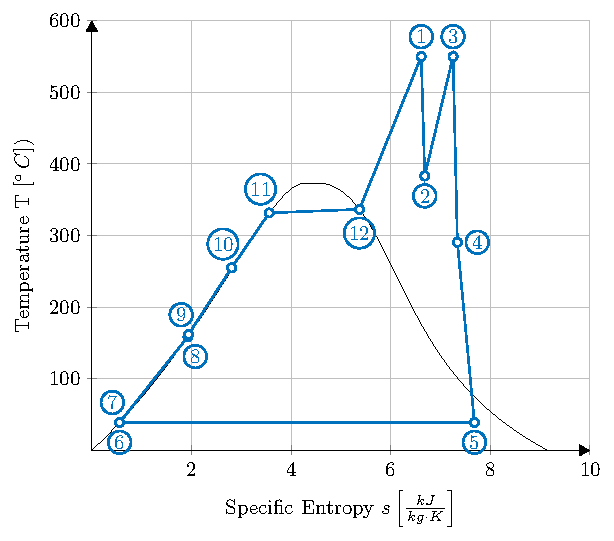
\includegraphics[scale=1.5]{all_points_plot_fig.pdf}
\end{figure}

\subsubsection*{Point 1)}
Point 1 is at \emph{high pressure turbine inlet}. We know its temperature $T_1=550\celsius$. We do not directly have the pressure $p_1$ but we can obtain it from the pressure drop at the super heater(SH) and evaporation pressure:
\begin{equation}
p_1 = p_{evap} \cdot \left( 1- \left. \frac{\Delta p}{p} \right\rvert_{SH} \right) = 128.8\,bar
\end{equation}
Now with the two parameters of temperature and pressure we can evaluate with \md also entropy and enthalpy functions of temperature and pressure:
\pointdatatable{1}{550}{128.8}{3472.6}{6.6142}
%
%
%
\subsubsection*{Point 2)}
\begin{wrapfigure}{L}{2cm}
    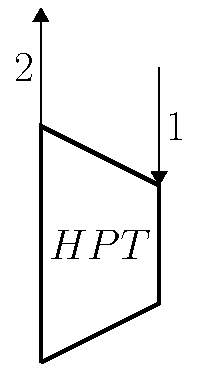
\includegraphics[scale=0.5]{hp_fig.pdf}
\end{wrapfigure}
Point 2 is at \emph{high pressure turbine outlet}. We know its pressure $p_2=42\,bar$. We do not directly have the temperature $T_2$ but we can obtain it from the definition of efficiency of the turbine:
\begin{equation}
\label{eq:eta_highp_turbine_iso}
\eta_T^{isoentropic} = \frac{h_1-h_2}{h_1-h_2^{IS}} = 87\%
\end{equation}
We don't know $h_2^{IS}$ but we can compute it from point 1 to point $2^{IS}$ considering an \emph{isoentropic process}:
\[\begin{cases}{}
p_2^{IS} = p_2 = 42 \,bar \\ 
s_2^{IS} = s_1 = 6.61 \kjkgk
\end{cases}\]
Now we can obtain from \md $h_2^{IS} = h(p_2^{IS},\ s_2^{IS}) = 3125.3 \kjkg$.
\\Reversing equation \ref{eq:eta_highp_turbine_iso} we can get $h_2$:
\begin{equation}
h_2=h_1-\eta_T^{iso} \cdot \left(h_1 - h_2^{IS} \right) = 3170.5 \kjkg
\end{equation}
With \md we finally evaluate $s_2 = s(p_2,\ h_2)$ and $T_2 = T(p_2,\ h_2)$ of point 2:
\pointdatatable{2}{383.165}{42}{3170.5}{6.6839}
%
%
%
\subsubsection*{Point 3)}
Point 3 is at \emph{intermediate pressure turbine inlet}. We know its temperature $T_3 = T_1 = 550 \celsius$. We do not directly have the pressure $p_2$ but we can obtain it from the pressure drop at the reheater(RH) and pressure at point 2:
\begin{equation}
p_3 = p_{2} \cdot \left( 1- \left. \frac{\Delta p}{p} \right\rvert_{RH} \right) = 38.64\,bar
\end{equation}
Now with the two parameters of Temperature and pressure we can evaluate with \md also entropy and enthalpy functions of temperature and pressure:
\pointdatatable{3}{550}{38.64}{3561.5}{7.2524}
%
%
%
\subsubsection*{Point 4)}
\begin{wrapfigure}{L}{2cm}
    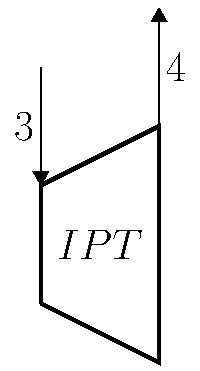
\includegraphics[scale=0.5]{ip_fig.pdf}
\end{wrapfigure}
Point 4 is at \emph{intermediate pressure turbine outlet} and \emph{low pressure turbine inlet}. We know its pressure $p_4=6\,bar$. We do not directly have the temperature $T_2$ but we can obtain it from the definition of efficiency of the turbine:
\begin{equation}
\label{eq:eta_intermediatep_turbine_iso}
\eta_T^{isoentropic} = \frac{h_3-h_4}{h_3-h_4^{IS}} = 91.5\%
\end{equation}
We don't know $h_4^{IS}$ but we can compute it from point 3 to point $4^{IS}$ considering an \emph{isoentropic process}:
\[\begin{cases}{}
p_4^{IS} = p_4 = 6 \,bar \\ 
s_4^{IS} = s_3 = 7.2524 \kjkgk
\end{cases}\]
Now we can obtain from \md $h_4^{IS} = h(p_4^{IS},\ s_4^{IS}) = 2994.4 \kjkg$.
\\Reversing equation \ref{eq:eta_intermediatep_turbine_iso} we can get $h_4$:
\begin{equation}
h_4=h_3-\eta_T^{iso} \cdot \left(h_3 - h_4^{IS} \right) = 3042.6 \kjkg
\end{equation}
With \md we finally evaluate $s_4 = s(p_4,\ h_4)$ and $T_4 = T(p_4,\ h4)$ of point 4:
\pointdatatable{4}{290.63}{6}{3042.6}{7.3397}
%
%
%
\subsubsection*{Point 5)}
\begin{wrapfigure}{L}{3cm}
    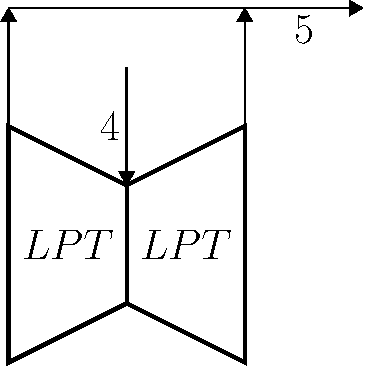
\includegraphics[scale=0.5]{lp_fig.pdf}
\end{wrapfigure}
Point 5 is at \emph{low pressure turbine outlet}. We know its pressure because is the condensation pressure $p_5=p_{COND}=0.07\,bar$. We do not directly have the temperature $T_5$ but we can obtain it like point 2 and 4 from the definition of efficiency of the turbine:
\begin{equation}
\label{eq:eta_lowp_turbine_iso}
\eta_T^{isoentropic} = \frac{h_4-h_5}{h_4-h_5^{IS}} = 86\%
\end{equation}
We don't know $h_5^{IS}$ but we can compute it from point 4 to point $5^{IS}$ considering an \emph{isoentropic process}:
\[\begin{cases}{}
p_5^{IS} = p_5 = 0.07 \,bar \\ 
s_5^{IS} = s_4 = 7.3397 \kjkgk
\end{cases}\]
Now we can obtain from \md $h_5^{IS} = h(p_5^{IS},\ s_5^{IS}) = 2279.9 \kjkg$.
\\Reversing equation \ref{eq:eta_lowp_turbine_iso} we can get $h_5$:
\begin{equation}
h_5=h_4-\eta_T^{iso} \cdot \left(h_4 - h_5^{IS} \right) = 2.3867 \kjkg
\end{equation}
Point 5 has a very low pressure and it fall in liquid-vapour region. So it is significant also to calculate the title of vapour.
With \md we finally evaluate $s_5 = s(p_5,\ h_5)$, $T_5 = T(p_5,\ h_5)$ and $\chi_5 = \chi(p_5,\ h_5)$ of point 5:
\pointdatatablechi{5}{39.0009}{0.07}{2386.7}{7.6817}{0.9232}
%
%
%
\subsubsection*{Point 6)}
Point 6 is at \emph{condenser outlet}. We know that when the flow goes out from the condenser is is a saturated liquid, and that the condenser is approximately isobaric, so we have $p_6=p_5=0.07\, bar$. We can get all missing properties from saturated liquid table: $T_6 = T^{liq}_{sat}(p_6)$, $h_6 = h^{liq}_{sat}(p_6)$, $s_6 = s^{liq}_{sat}(p_6)$ and $\rho_6 = \rho^{liq}_{sat}(p_6)$ .
\pointdatatablerho{6}{39.0009}{128.8}{163.3655}{0.5591}{992.55}
%
%
%
\subsubsection*{Point 7)}
Point 7 is at \emph{the outlet of the first pump} and \emph{deaerator inlet}. We know its pressure because point 7 is in contact with point 4$^{extr}$ through the isobaric deaerator, so $p_7=p_4^{extr}=p_4=6\, bar$. 
We do not directly have the enthalpy $h_7$ but we can obtain it from the definition of efficiency of the pump:
\begin{equation}
\label{eq:eta_pump1_iso}
\eta_{p_1}^{hydraulic} = \frac{h_7^{IS}-h_6}{h_7-h_6} = 84\%
\end{equation}
We don't know $h_7^{IS}$ and we can get it in two ways:
%
\begin{itemize}
\item with subcooled liquid tables or tools considering an \emph{isoentropic process} between 6 and 7$^{IS}$  considering that \[\begin{cases}{}
p_7^{IS} = p_7 = 6 \,bar \\ 
s_7^{IS} = s_6 = 0.5591 \kjkgk
\end{cases}\]
\item estimating $h_7^{IS}-h_6 \approx \frac{p_7-p_6}{\rho_6}$ with hypothesis of incompressible flow and density constant with temperature and pressure.
\end{itemize}
%
Reverting equation \ref{eq:eta_pump1_iso} with the second stated approach we get:
\begin{equation}
\label{eq:entalpy_point7}
h_7 = h_6 + \frac{p_7-p_6}{\rho_6 \cdot \eta_{hyd}} = 164.08 \kjkg
\end{equation}
With the same hypothesis we evaluate $T_7$ and $s_7$:
%
\begin{align}
du       &= dh-\frac{dp}{\rho} = c_L \cdot dT,\\
\Delta T &= \frac{\Delta u}{c_L} = T_7 - T_6\\
\Delta u &= \Delta h-\frac{\Delta p}{\rho} = \frac{\Delta h^{IS}}{\eta_{hyd}} - \frac{\Delta p}{\rho} \\
         &\approx \frac{\Delta p}{\rho \cdot \eta_{hyd}} - \frac{\Delta p}{\rho} 
         =\frac{\Delta p}{\rho} \cdot \left( \frac{1}{\eta_{hyd}} -1 \right) \\
T_7      &= T_6 + \frac{\Delta u}{c_L} 
= T_6 + \frac{\Delta p}{\rho \cdot c_L} \cdot \left( \frac{1}{\eta_{hyd}} -1 \right)
\label{eq:temperature_point7}
\end{align}
%
\begin{align}
Tds      &= du+p\cancel{dv} =c_L \cdot DT\\
ds       &= c_L \cdot \frac{dT}{T}\\
\Delta s &= s_7 - s_6 = c_L \cdot \log \left( \frac{dT}{T} \right)\\
s_7      &= s_6 + c_L \cdot \log \left( \frac{dT}{T} \right)
\label{eq:entropy_point7}
\end{align}
%
Finally we find:
\pointdatatable{7}{39.0607}{6}{164.08}{0.5597}
%
%
%
\subsubsection*{Point 8)}
Point 8 is at \emph{outlet of deaerator}. We know that when the flow goes out from the deaerator is is a saturated liquid, and that deareator is approximately isobaric, so we have $p_8=6\, bar$.We can get all missing properties from saturated liquid table: $T_8 = T^{liq}_{sat}(p_8)$, $h_8 = h^{liq}_{sat}(p_8)$, $s_8 = s^{liq}_{sat}(p_8)$ and $\rho_8 = \rho^{liq}_{sat}(p_8)$ .
\pointdatatablerho{8}{158.83}{128.8}{670.50}{1.9311}{908.5657}
%
%
%
\subsubsection*{Point 9)}
Point 9 is at \emph{the outlet of the second pump}. We can simply evaluate its pressure because we know the pressure drop in economizer and that RB is approximately isobaric. So:
\begin{equation}
p_9 = \frac{p_{EVAP}}{1-\left. \frac{\Delta p}{p} \right\rvert_{ECO} } = 175\, bar
\end{equation}
We do not directly have the enthalpy $h_9$ but we can obtain it from the definition of efficiency of the pump and with the same hypothesis of equation \ref{eq:entalpy_point7}
\begin{equation}
h_9 = h_8 + \frac{p_9-p_8}{\rho_8 \cdot \eta_{hyd}} = 692.645 \kjkg
\end{equation}
And in the same way of point 7 we can estimate $T_9$ and $s_9$ from equations \ref{eq:temperature_point7} and \ref{eq:entropy_point7}:
\begin{align}
T_9 &= T_8 + \frac{\Delta u}{c_L}\\
s_9 &= s_8 + c_L \cdot \log \left( \frac{dT}{T} \right)
\end{align}
Finally we find:
\pointdatatable{9}{161.6521}{175}{692.6450}{1.9396}
%
%
%
\subsubsection*{Point 10)}
Point 10 is at \emph{regenerator outlet} and \emph{economizer inlet}. We have from data $T_{10}=255 \celsius$ and moreover $P_9=P_{10}=175\, bar$ assuming the regenerator approximately isobaric. From the regenerator the flow is a subcooled liquid. We have the two main properties so we are able with \md for subcooled liquid to find all the missing properties needed. Alternatively we may use the following approximations:
\begin{numcases}{}
\label{eq:enthalpy_point10}
h_{10} \approx h^{liq}_{sat}(T_{10}) + \upsilon^{liq}_{sat}(T_{10}) \cdot \left( p_{10} - p_{sat}(T_{10}) \right) \\ 
\label{eq:entropy_point10}
s_{10} \approx s^{liq}_{sat}(T_{10}) 
\end{numcases}
\pointdatatable{10}{255}{175}{1109.9}{2.8074}
%
%
%
\subsubsection*{Point 11)}
Point 11 is at \emph{economizer outlet}. We have from data $p_{11}=p_{EVAP}=140\, bar$ and the temperature is $5 \celsius$ lower than evaporation temperature so $T_{11}=T_{EVAP}-5 \celsius=T_{sat}(p_{EVAP})-5 \celsius=331.67 \celsius$. As point 10, point 11's flow is subcooled liquid than we can use approximation of equations \ref{eq:enthalpy_point10} and \ref{eq:entropy_point10} to compute all properties:
\pointdatatable{11}{331.67}{140}{1533.6}{3.5616}
%
%
%
\subsubsection*{Point 12)}
Point 12 is at \emph{evaporator outlet} and \emph{superheat inlet}. We know that when the flow goes out from the evaporator it is saturated vapour, so we have $p_{12}=p_{EVAP}=140\, bar$. We can get all missing properties from saturated vapour table: $T_{12} = T^{vap}_{sat}(p_{12})$, $h_{12} = h^{vap}_{sat}(p_{12})$, $s_{12} = s^{vap}_{sat}(p_{12})$ and $\rho_{12} = \rho^{vap}_{sat}(p_{12})$ .
\pointdatatablerho{12}{336.67}{140}{2638.1}{5.3730}{87.03}
%
%
%
\subsubsection*{Point \boldsymbol{ $2_{DR}$})}
\begin{figure}[h]
  \caption{Regenerator flow Scheme.}
  \centering
  \usetikzlibrary{decorations.pathmorphing}
\usetikzlibrary{decorations.markings}
\usetikzlibrary{decorations.pathmorphing}
\usetikzlibrary{arrows}
\begin{tikzpicture}[>=triangle 60]
% rectangle
\draw[very thick] (0,0) rectangle (5,3);
% cold end
\draw[fill=blue!30,draw=blue,thick] (6.2,1.5) ellipse (0.9 and 1.2);
\node[blue,right] at (7,2) {Cold\ End};
% hot end
\draw[fill=red!30,draw=red,thick] (-1.5,1.5) ellipse (0.9 and 1.2);
\node[red,left] at (-2.3,2.02) {Hot\ End};
% air line
\draw[]  (-1,2)--(1,2);
\draw[decorate,decoration=zigzag] (1,2)--(4,2);
\draw[->]  (4,2)--(6,2);
% flue gas linetriangle 60
\draw[<-]  (-1,1)--(1,1);
\draw[decorate,decoration=zigzag] (1,1)--(4,1);
\draw[]  (4,1)--(6,1);
%
\node[red,left] at (-1,2) {$2_{extr}$};
\node[red,left] at (-1,1) {$10$};
%
\node[blue,right] at (6,2) {$2_{DR}$};
\node[blue,right] at (6,1) {$9$};
% heat transfer
\draw[red, decorate,decoration={snake,post length=1.5mm}, ->] (2.5,2.5)--(2.5,0.5);
%\draw[red,<-]  (2.5,0.5)--(2.5,0.5);
\node[red,left] at (2.4,2.6) {$\dot{Q}$};
\end{tikzpicture}
\end{figure}
Point $2_{DR}$ is at \emph{regenerator outlet} and \emph{deaerator inlet}. We have from data $T_{2_{DR}}=T_9-5 \celsius = 166.65 \celsius$. Assuming that the regenerator is isobaric we have that $p_{2_{DR}} = p_{4_{extr}} = p_4=42\, bar$. From the regenerator the flow is a subcooled liquid. We have the two main properties so we are able with \md for subcooled liquid to find all the missing properties needed. Alternatively we may use the following approximations like point 7 and 10:
\begin{numcases}{}
\label{eq:enthalpy_point2dr}
h_{10} \approx h^{liq}_{sat}(T_{10}) + \upsilon^{liq}_{sat}(T_{10}) \cdot \left( p_{10} - p_{sat}(T_{10}) \right) \\ 
\label{eq:entropy_point2dr}
s_{10} \approx s^{liq}_{sat}(T_{10}) 
\end{numcases}
\pointdatatable{2_{DR}}{166.65}{42}{706.51}{2.0046}

\input{table_all_properties}
%
%
%
\subsection{Calculation of the mass flow rates of each mass stream of the steam cycle}
In order to evaluate the mass flow rates $\dot{m_1}$ and $\dot{m_{extr}}$, we need to apply the mass conservation law in combination with the energy balance to some section (control volume) of the steam cycle (remembering that we deal with an open system in steady state process). 
\begin{itemize}
\item With energy balance at the boiler and energy balance at the regenerator we can write:
%
\begin{numcases}{}
\dot{H}_{SH} + \dot{H}_{EVAP} + \dot{H}_{ECO} + \dot{H}_{RH} = \dot{Q}^{IN}_{cycle}\\
\dot{H}_{2 \rightarrow 2_{DR}} = \dot{H}_{9 \rightarrow 10}
\end{numcases}
%
\begin{numcases}{}
\dot{m}_{1}( \overbrace{h_1-h_{12}}^{SH} + 
		     \overbrace{h_{12}-h_{11}}^{EVAP}+ 
		     \overbrace{h_{11}-h_{10}}^{ECO} ) +  
\dot{m}_{2}(\overbrace{h_{3}-h_{2}}^{RH})
= \dot{Q}^{IN}_{cycle}\\
\dot{m}_{2_{extr}}(h_{2_{extr}}-h_{2{DR}})
= \dot{m}_{1}(h_{10}-h_{9})\\
\dot{m}_{1} = \dot{m}_{2} + \dot{m}_{2_{extr}}
\end{numcases}

We have computed all the enthalpy before so we can solve the linear system and we are able to find all the 3 unknown mass flow rates:
\begin{center}
\tabulinesep=1.2mm
\begin{tabu}{|c|c|c|}
\hline
$ \dot{m}_{1} $ & $ \dot{m}_{2} $ & $ \dot{m}_{2_{extr}} $\\ \hline
$ 372.09 \kgs $	& $ 309.08 \kgs $ & $ 63.01 \kgs $ \\ \hline
\end{tabu}
\end{center}

\item With energy balance at the reaerator and mass flow rates balance at the reaerator we can write:
%
\begin{figure}[h]
	\centering
    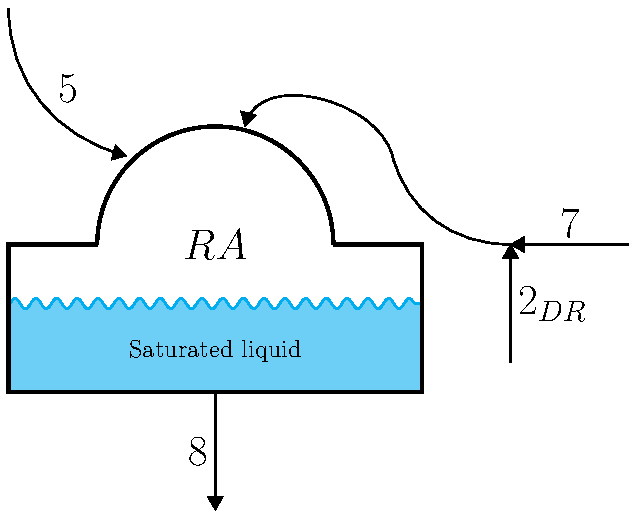
\includegraphics[scale=0.6]{RA_fig.pdf}
    \caption{Reaerator flow scheme.}
\end{figure}
\begin{numcases}{}
\dot{m}_8h_8 = \dot{m}_{4_{extr}}h_{4_{extr}} + \dot{m}_7h_7 + \dot{m}_{2_{DR}}h_{2_{DR}}\\
\dot{m}_7 = \dot{m}_1 - \dot{m}_{2_{DR}} - \dot{m}_{4_{extr}}
\end{numcases}
%
Where the only unknowns are $\dot{m}_{4_{extr}}$ and $\dot{m}_7$.
We have already computed enthalpy of every point so we can solve the linear system and we are able to find all the 2 unknown mass flow rates:
\begin{center}
\tabulinesep=1.2mm
\begin{tabu}{|c|c|}
\hline
$ \dot{m}_{7} $ & $ \dot{m}_{4_{extr}} $\\ \hline
$ 255.49 \kgs $ & $ 53.59 \kgs $\\ \hline
\end{tabu}
\end{center}
\end{itemize}

\subsection{Evaluation of cycle performances}
We can compute all the performance parameters for the steam cycle:
\begin{itemize}
\item Blade power output of the turbine (that is the inner power output, or equivalently the turbine power without mechanical losses): 
\begin{equation}
\dot{W}_T = \dot{m}_1(h_1-h_2) + 
			\dot{m}_2(h_3-h_4) +
			\dot{m}_4(h_4-h_5) = 440.39 \kw
\end{equation}
%
\item Blade power output of the condensate extraction pump:
\begin{equation}
\dot{W}_{P1} = \dot{m}_6(h_7-h_6) = 181.715 \kw
\end{equation}
%
\item Blade power output of the feedwater pump:
\begin{equation}
\dot{W}_{P2} = \dot{m}_8(h_9-h_8) = 8.240 \kw
\end{equation}
%
\item \underline{Thermal power rejected from the condenser}:
\begin{equation}
\dot{Q}_{condenser} = \dot{m}_6(h_5-h_6) = 568.04 \kw
\end{equation}
%
\item \underline{Gross electrical power output (Steam Turbine)}, that is the electric power at the electric generator, accounting for the mechanical and electric conversion losses 
\begin{equation}
\dot{W}^{gross}_T = \dot{W}_T \cdot \eta^M_T \cdot \eta^E_T = 425.10 \kw
\end{equation}
%
\item \underline{Net electrical power output of the cycle}, which accounts for the electric consumption not only in the steam cycle (condenser and feedwater pumps) but also plant auxiliaries electric consumption $W_{aux}$ (fans supplying air and evacuating flue gases to the stack, heat rejection, etc.):  
\begin{equation}
\dot{W}^{net}_{cycle} = \dot{W}^{gross}_T - \frac{\dot{W}_{P1}}{\eta^M_{P1}} - \frac{\dot{W}_{P2}}{\eta^M_{P2}} = 415.75 \kw
\end{equation}
%
\item \underline{Thermodynamic efficiency of the cycle}, which is defined as the ratio between the net fluid power of the cycles before any mechanical losses and the thermal power input into the cycle:
\begin{equation}
\eta_{cycle} = \frac{\dot{W}_T - \dot{W}_{P1} - \dot{W}_{P1}}{\dot{Q}^{IN}_{cycle}}
 = 43.20 \%
\end{equation}
%
\item \underline{Net electrical power output of the power plant}:
\begin{equation}
\dot{W}^{net}_{plant} = \dot{W}^{net}_{cycle} - 3.2\% \cdot \dot{W}^{gross}_T = 402.14 \kw 
\end{equation}
%
\item \underline{Net electrical efficiency of the power plant}, which is defined referred to the thermal input to the plant (associated to the fuel) as: 
\begin{equation}
\eta_{plant} = \eta_{boiler} \cdot \frac{\dot{W}^{net}_{plant}}{\dot{Q}^{IN}_{cycle}}
 = 38.16 \%
\end{equation}
\end{itemize}

\subsection{Representation of T-Q diagram of the surface feedwater preheater RB}
At this point, only the inlet and outlet thermodynamic conditions of both of the streams are known. In order to evaluate the T-Q profiles (temperature-heat exchanged) of hot ($2_{extr}-2_{DR}$) and cold (9-10) streams, three assumptions can be outlined:
\begin{enumerate}
\item The heat exchanger is supposed to be arranged in a \emph{countercurrent} configuration;
\item \emph{Three different sections} can be identified along the feedwater preheater:
	\begin{enumerate}
	\item De-superheating of the bled steam ($RB_I$);
	\item Condensation of the bled stream ($RB_{II}$);
	\item Sub-cooling of the bled stream ($RB_{II}$);
	\end{enumerate}
\item In each section, we suppose that the streams have a \emph{constant thermal capacity}.
\end{enumerate}

\begin{equation}
\dot{Q}_{RB}^{I} = \dot{m}_9 \cdot (h_{10}-h_{9b})
= \dot{m}_9 \cdot \overline{c_p} \cdot (T_{10}-T_{9b})
= \dot{m}_{2_{extr}} \cdot (h_{2_{extr}} - h^{vap}_{sat}(p_2))
= 23.35 \kw
\end{equation}
But with the assumption of $c_p$ approximately constant we can evaluate a medium value between 9 and 10:
\begin{equation}
\dot{Q}_{RB} = \dot{m}_9 \cdot (h_{10}-h_{9})
= \dot{m}_9 \cdot \overline{c_p} \cdot (T_{10}-T_{9}) = 155.27 \kw
\end{equation}
\begin{equation}
\dot{m}_9 \cdot \overline{c_p} = \frac{\dot{Q}_{RB}}{T_{10}-T_{9}} = 1663.3 \kjkg 
\end{equation}
\begin{equation}
T_{9b} = T_{10} - \frac{\dot{Q}_{RB}^{I}}{\dot{m}_9 \cdot \overline{c_p}}
= T_{10} - \frac{\dot{m}_{2_{extr}} \cdot (h_{2_{extr}} - h^{vap}_{sat}(p_2)) }{\dot{m}_9 \cdot \overline{c_p}} =  240.96 \celsius
\end{equation}
We can similarly proceed from point b to point a:
\begin{equation}
\dot{Q}_{RB}^{II} = \dot{m}_9 \cdot (h_{9b}-h_{9a})
= \dot{m}_9 \cdot \overline{c_p} \cdot (T_{9b}-T_{9a})
= \dot{m}_{2_{extr}} \cdot (h^{vap}_{sat}(p_2) - h^{liq}_{sat}(p_2))
= 10.70 \kw
\end{equation}
\begin{equation}
T_{9a} = T_{9b} - \frac{\dot{Q}_{RB}^{II}}{\dot{m}_9 \cdot \overline{c_p}}
= T_{10} - \frac{\dot{m}_{2_{extr}} \cdot (h^{vap}_{sat}(p_2) - h^{liq}_{sat}(p_2)) }{\dot{m}_9 \cdot \overline{c_p}} =   176.62 \celsius
\end{equation}

The only missing data is the temperature of saturation at $p_2$; with \md we can find it: $T_{sat} = 253.27 \celsius$

Now we can plot Q-T diagram:

\begin{figure}[h]
\centering
    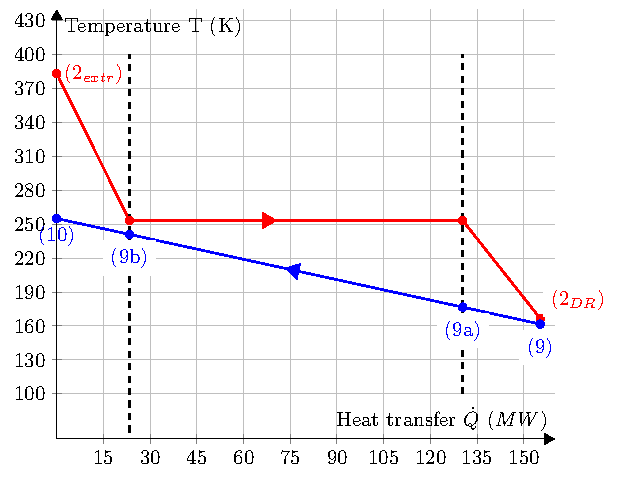
\includegraphics[width=0.9\textwidth]{TQ_plot_fig.pdf}
\end{figure}

\end{document}
